\documentclass[10pt,a4paper]{article}
\usepackage[margin=21mm]{geometry}
\usepackage[T1]{fontenc}
\usepackage[utf8]{inputenc}
\usepackage{lmodern,amsmath,amssymb,booktabs,graphicx,array,xcolor,hyperref}
\hypersetup{colorlinks=true,linkcolor=blue,urlcolor=blue}
\newcommand{\vswirl}{\mathbf{v}_{\!\boldsymbol{\circlearrowleft}}}
\newcommand{\rhof}{\rho_{\!f}}
\newcommand{\rc}{r_c}
\title{\textbf{A070 (provisional) --- Absolute Time, Swirl Clocks and Operational Distance}\\[1mm]\large Executed analytical / numerical falsifier pilot v0.1.0}
\author{SST Workbench --- exploratory science instance}
\date{18 October 2026\\\textbf{DEVELOPMENT / NOT CERTIFIED / NOT PHYSICALLY BLIND}}
\begin{document}\maketitle
\noindent\textbf{Status and limitations.} This is a self-contained model-diagnostic pilot, not a frozen SST Framework v1.0.7 instance. Source-native finite-core PKLSA input, experimentally determined photon propagation, a physical rod model and astronomical likelihood tests are not available here. Synthetic-controls cannot certify gravity or cosmology. The catalog ID A070 is unverified against local Workbench registries.\par
\section{The fundamental distinction: absolute and operational quantities}
The SST hypothesis is a Euclidean, incompressible fluid evolving in one absolute time parameter $t$:
\begin{equation}\nabla\cdot\mathbf u=0,\qquad \frac{D\mathbf u}{Dt}=-\frac{\nabla p}{\rhof}.
\end{equation}
Clock $i$ has internal vortex phase $\theta_i$ and inferred local Swirl-Clock time:
\begin{equation}\label{eq:clock}\frac{d\theta_i}{dt}=\Omega_i(t),\qquad \frac{d\tau_i}{dt}=f_i(t)=\frac{\Omega_i(t)}{\Omega_{i,0}},\qquad \tau_i(t)=\int_0^t f_i(s)\,ds.
\end{equation}
Euclidean separation $D_{\rm abs}$, two-way radar separation $D_{\rm rad}$, and rod-count separation $D_{\rm rod}$ are \emph{distinct physical constructions}. Inferring the last two requires independent signal/rod physics. Absolute time is not a universal synchrony requirement for atomic clocks.
\section{An exact stretching Euler control}
Use the nonuniform affine velocity field
\begin{equation}\label{eq:affine}
\mathbf u=\begin{pmatrix}-sx/2-\Omega(t)y\\\Omega(t)x-sy/2\\sz\end{pmatrix},\qquad
\Omega(t)=\Omega_0e^{st},\quad s>0.
\end{equation}
It obeys $\nabla\cdot\mathbf u=0$ and $\boldsymbol\omega=(0,0,2\Omega)$. Direct substitution into the Euler equation yields the exact pressure
\begin{equation}\label{eq:p}
p=p_0-\frac{\rhof}{2}\left[\left(\frac{s^2}{4}-\Omega(t)^2\right)(x^2+y^2)+s^2z^2\right].
\end{equation}
The moving core is stretched along $z$ and compressed transversely, preserving local material volume:
\begin{equation}\label{eq:stretch}L_z/L_{z0}=e^{st},\quad a/a_0=e^{-st/2},\quad\Omega/\Omega_0=e^{st}.
\end{equation}
The analytic and Python FP64 acceleration matrices match in the reported benchmark. \textbf{Critical caveat:} Eq.~\eqref{eq:affine} is not a finite-energy global vortex network or a dynamically certified knotted filament. Its infinite-domain behavior makes it suitable only as an analytic control. For numerical illustration only, $\Omega_0=|\vswirl|/\rc=7.76344\times10^{20}\,\mathrm{s}^{-1}$, $s=0.12/\mathrm{Gyr}=3.80257\times10^{-18}\,\mathrm{s}^{-1}$ and $\rhof=7\times10^{-7}\,\mathrm{kg\,m^{-3}}$. The clock frequency is a hypothesis about core rotation, not a resolved PKLSA mode.\par
\section{Gate results: absolute distance versus clock and rod measures}
\textbf{G1: Clock-only acceleration.} For fixed $D_{\rm abs}=D_0$, under a constant absolute-coordinate signal speed $c$ and \emph{short-baseline/quasi-static} two-way ranging:
\begin{equation}\tau=\frac{e^{st}-1}{s},\qquad D_{\rm rad}=f(t)D_0=D_0(1+s\tau),\qquad\boxed{\frac{d^2D_{\rm rad}}{d\tau^2}=0.}
\end{equation}
Thus this particular physical exponential stretching law does \textbf{not} produce an accelerating operational distance from a fixed Euclidean separation. A derivative-on-grid test has maximum dimensionless second derivative $5.42\times10^{-12}$ after rescaling distance by $D_0$ and local time by a Gyr. This result does not apply to cosmological light-travel distances, where full signal and clock history must be integrated.\par
\textbf{G2: Rod--clock--signal closure.} If a material rod is the core diameter $a(t)$, measured rod-count distance is $D_{\rm rod}=D_{\rm abs}e^{st/2}$, whereas radar gives $D_{\rm rad}=D_{\rm abs}e^{st}$. Therefore
\begin{equation}\frac{c_{\rm measured}}{c}=\frac{1}{f(a/a_0)}=e^{-st/2}.\end{equation}
At one Gyr, with $s\,\mathrm{Gyr}=0.12$, this gives $0.9417645$: a $5.82\%$ local measured speed drift under this \emph{specific} trio of assumptions. A consistent SST photon law or different physical rod may change this; no unconditional falsification is claimed.
\begin{figure}[h!]\centering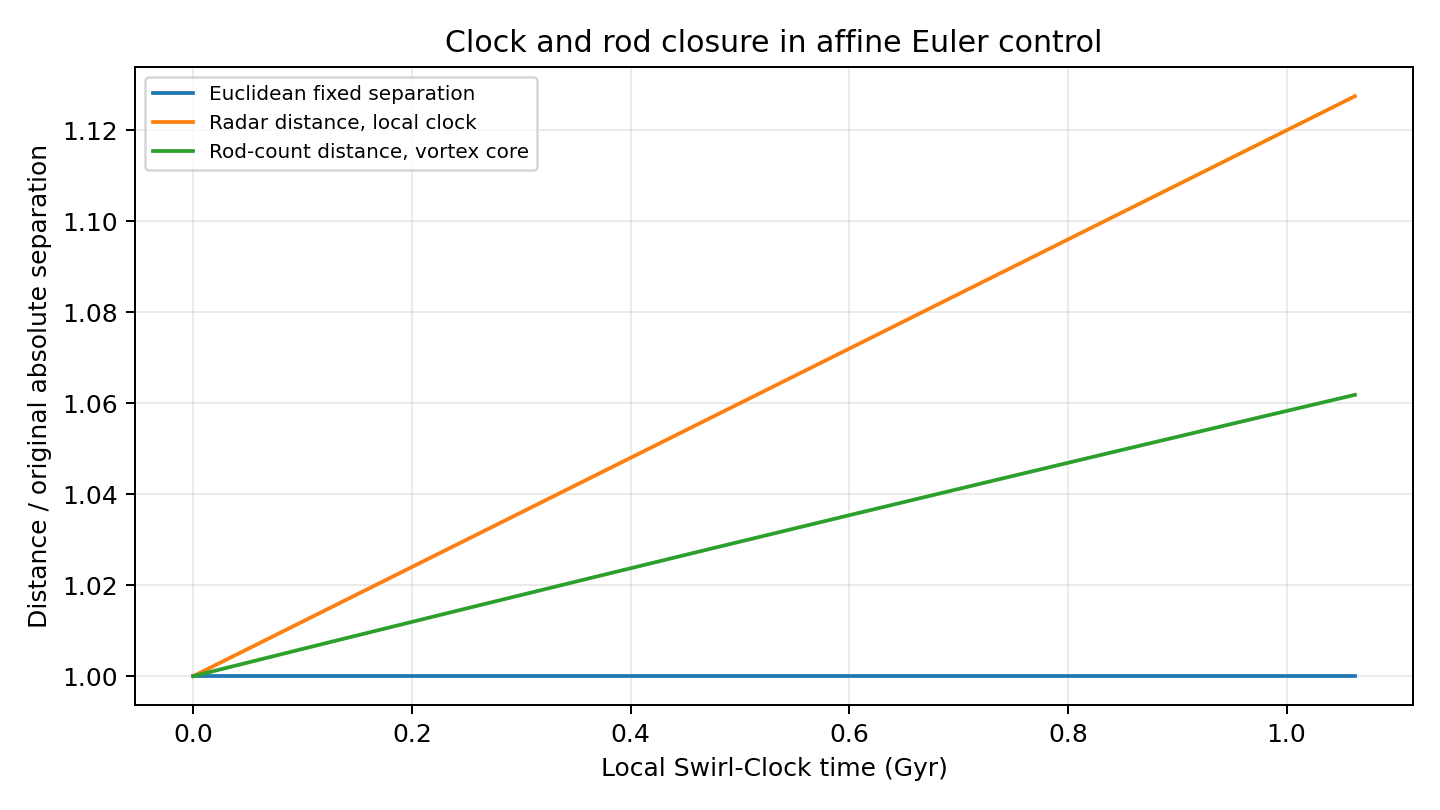
\includegraphics[width=.86\linewidth]{figures/clock_rod.png}\caption{The same fixed Euclidean baseline can have different operational lengths under two independently proposed measurement recipes.}\end{figure}
\clearpage
\textbf{G3: Isotropy.} A pair of material tracers separated along the $z$ axis moves as $D_z=D_0e^{st}$, while a transverse pair has $D_x=D_0e^{-st/2}$. The volume ratio $D_zD_x^2/D_0^3=1$. Radar estimates grow as $e^{2st}$ in $z$ but $e^{st/2}$ transversely, so a generically \emph{isotropic} apparent expansion is not recovered. In local time, $D_{{\rm rad},z}=D_0(1+s\tau)^2$ and $D_{{\rm rad},x}=D_0(1+s\tau)^{1/2}$; these have opposite signs of second derivative.
\begin{figure}[h!]\centering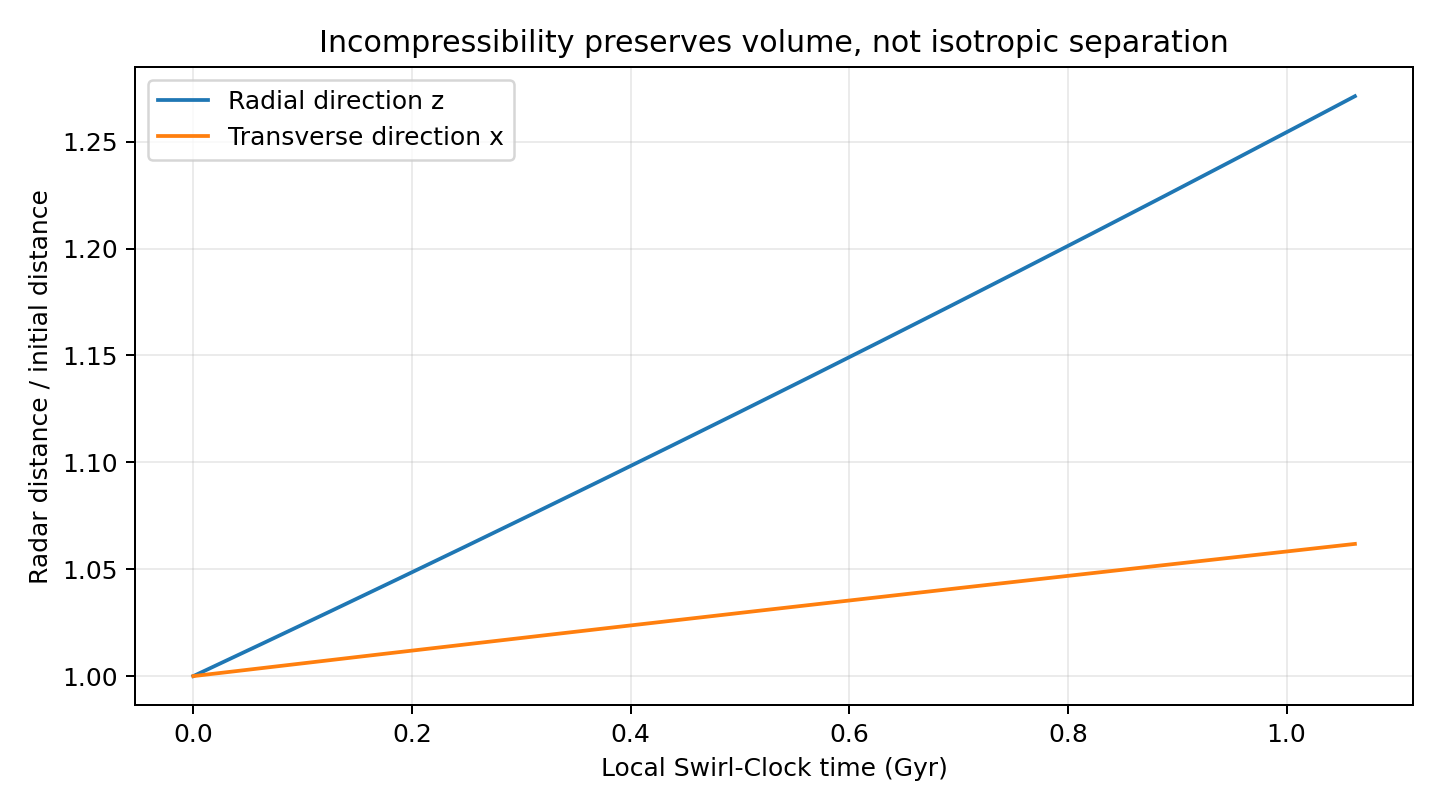
\includegraphics[width=.86\linewidth]{figures/anisotropy.png}\caption{An exact incompressible affine flow generates axis-dependent separations: longitudinal expansion and transverse contraction.}\end{figure}
\section{Optical-distance hypothesis: synthetic EdS against synthetic flat $\Lambda$CDM}
A static background does not have a derived SST photon/atomic-redshift law yet. Instead, as a \emph{mathematical identifiability test}, compare the standard toy curves (not observations):
\begin{equation}
D_L(z)=(1+z)\frac{c}{H_0}\int_0^z\frac{dq}{E(q)},\quad E_{\rm EdS}=(1+z)^{3/2},\quad E_{\Lambda{\rm CDM}}=\sqrt{0.3(1+z)^3+0.7}.
\end{equation}
For phenomenological optical depth $\mathcal T(z)$, $F_{\rm obs}=F_{\rm EdS}e^{-\mathcal T(z)}$ and $D_{L,\rm obs}=D_{L,\rm EdS}e^{\mathcal T/2}$. The exactly constructed target-dependent law is
\begin{equation}\label{eq:opt}\mathcal T_*(z)=2\ln\left(\frac{D_{L,\Lambda{\rm CDM}}}{D_{L,\rm EdS}}\right).
\end{equation}
It matches by construction and therefore has no predictive validity. At $z=1$, $\mathcal T_*(1)=0.550574$, corresponding to an extra $42.34\%$ flux suppression compared to EdS and a distance-duality factor $\eta=e^{\mathcal T_*/2}=1.31691$ (if $D_A$ remains unchanged). Such large effects require independent observational testing.
\paragraph{G5: Low-$z$ fit and independent high-$z$ synthetic holdout.}
A restrictive one-parameter response $\mathcal T(z)=\alpha z$ was fit at $z\in\{0.1,0.2,0.35,0.5\}$ and evaluated at $z\in\{0.8,1.0,1.5,2.0\}$ without refitting. It gives $\alpha=0.778159$ and held-out RMS magnitude residual $0.553317\,\mathrm{mag}$, against exploratory preset acceptance $0.020\,\mathrm{mag}$. This \textbf{fails the synthetic holdout}, not a real cosmic observation. EdS and $\Lambda$CDM already both have their own cosmological time dilation; opacity alone is not an SST origin of redshift or time stretching.
\begin{figure}[h!]\centering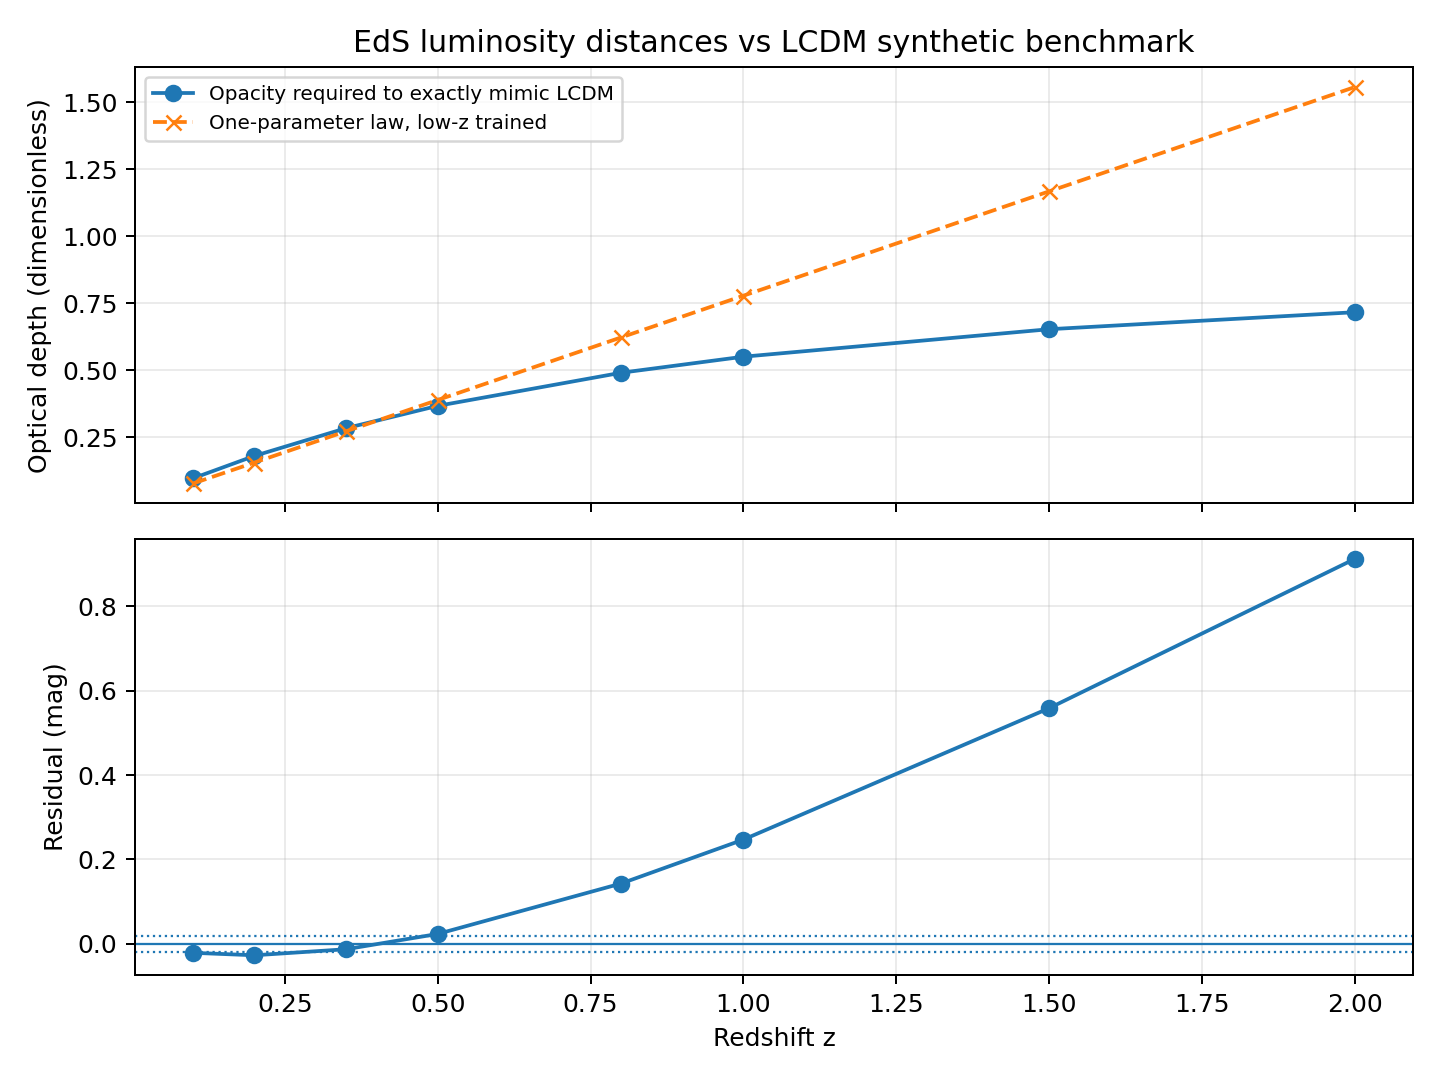
\includegraphics[width=.84\linewidth]{figures/opacity_holdout.png}\caption{Exactly constructed target-dependent opacity (identity only) compared with the held-out extrapolation of one simple opacity law.}\end{figure}
\section{Audit-grade gate ledger}
\begin{center}\small\begin{tabular}{p{11mm}p{39mm}p{88mm}}\toprule Gate & Numerical result & Scope / status\\\midrule
G0 & PASS\_REFERENCE & Exact solenoidal affine Euler control, not a finite-energy 3D knot.\\
G1 & NULL\_RETAINED & Clock-only positive acceleration fails for fixed absolute baseline in this model.\\
G2 & FAIL\_MODEL\_CLOSURE & Clock + core radius + constant absolute signal speed imply 5.82\% local signal-speed variation over chosen benchmark.\\
G3 & FAIL\_ISOTROPIC & Axial expansion and transverse contraction, material volume exactly preserved.\\
G4 & PASS\_IDENTITY\_ONLY & Target-constructed opacity reproduces target by definition.\\
G5 & FAIL\_SYNTHETIC\_HOLDOUT & $0.553317$ mag holdout RMS exceeds $0.020$ mag synthetic threshold.\\
G6 & UNRESOLVED & No resolved source-native finite-core PKLSA and no independent photon/rod physics or real observation likelihood.\\\bottomrule\end{tabular}\end{center}
\section{Next physically discriminating test}
Generate a frozen v1.0.7 instance only after audit of the Workbench registry ID. Supply source-native finite-core vortex seeds and independently propagated internal perturbation modes. Evolve them in common absolute $t$; determine $f_i(t)$ from modes, not a fitted relativistic factor; determine material length standards from resolved structure and light propagation from an independently specified field equation. Separate statistical evidence for distance--redshift, redshift--time dilation, BAO angular/radial distances and lensing. Never promote a synthetic-control PASS to a physical SST claim.\par
The framework v1.0.7 reference was verified in Drive on this date; its frozen generator, blind policies, CPU certification and PDF reporting were \emph{not} executed as part of this standalone pilot. The code is source-ready for controlled integration.
\section*{References}\begin{thebibliography}{9}
\bibitem{Batchelor1967} G. K. Batchelor (1967), \emph{An Introduction to Fluid Dynamics}, Cambridge University Press. DOI: \href{https://doi.org/10.1017/CBO9780511800955}{10.1017/CBO9780511800955}.
\bibitem{Etherington1933} I. M. H. Etherington (1933), ``On the Definition of Distance in General Relativity,'' \emph{Philosophical Magazine} \textbf{15}, 761--773. DOI: \href{https://doi.org/10.1080/14786443309462220}{10.1080/14786443309462220}.
\bibitem{Riess1998} A. G. Riess et al. (1998), ``Observational Evidence from Supernovae for an Accelerating Universe and a Cosmological Constant,'' \emph{Astronomical Journal} \textbf{116}, 1009--1038. DOI: \href{https://doi.org/10.1086/300499}{10.1086/300499}.
\bibitem{DESI2026} DESI Collaboration, \emph{DESI DR2 cosmological results and documentation} (2025--2026), \url{https://data.desi.lbl.gov/doc/papers/}.
\bibitem{Chaudhary2026} H. Chaudhary, S. Capozziello, V. K. Sharma et al. (2026), ``Evidence for evolving dark energy from DESI DR2 BAO and Pantheon$^+$, DES-Dovekie, and Union3,'' \emph{European Physical Journal C} \textbf{86}, 564. DOI: \href{https://doi.org/10.1140/epjc/s10052-026-15806-w}{10.1140/epjc/s10052-026-15806-w}.
\end{thebibliography}
\end{document}
